\documentclass[a4paper,onecolumn]{report}
\usepackage{caption}
\usepackage{subcaption}
\usepackage{setspace}
\usepackage{amssymb}
\usepackage[fleqn]{amsmath}
\usepackage{apacite}
\usepackage{graphicx}
\usepackage{color}
\usepackage{float}
\usepackage[toc,page]{appendix}
\usepackage[nottoc]{tocbibind}
\usepackage{titlesec}
\usepackage{float}
\usepackage{color}
\usepackage{setspace}
\usepackage{comment}
\usepackage{url}
\titleformat{\chapter}{\normalfont\huge}{\thechapter.}{15pt}{\huge}
\renewcommand*{\familydefault}{\sfdefault}
\hyphenpenalty=5000 
\tolerance=1000

\usepackage[a4paper]{geometry}
\voffset=-50pt
\hoffset=0pt
\topmargin = 0pt
\textwidth = 450pt
\textheight = 700pt
\marginparwidth = 10pt
\oddsidemargin = 5pt
\topmargin = 1pt
\graphicspath{ {/images/} }

\setcounter{tocdepth}{2}

\begin{document}

%----------------------------------------------------------------------------------------
%	TITLE SECTION
%----------------------------------------------------------------------------------------

\begin{titlepage}

\newgeometry{top=3in}

\newcommand{\HRule}{\rule{\linewidth}{0.5mm}}
\newcommand{\horrule}[1]{\rule{\linewidth}{#1}}

\center % Center everything on the page

\textsc{\small DELFT UNIVERSITY of TECHNOLOGY}\\[2.5cm] % Name of your university/college

\textsc{\LARGE Artificial Neural Networks}\\[0.5cm] % Major heading such as course name

\HRule \\[0.1cm]
\begin{spacing}{1.6}
{ \huge PROJECT REPORT}\\[-0.4cm] % Title of your document
\end{spacing}
\HRule \\[1.5cm]

\begin{minipage}{0.4\textwidth}
\begin{flushleft} \large
\emph{Authors:}\\
Michiel \textsc{Bongaerts\\}
Marjolein \textsc{Nanninga}\\
Tung \textsc{Phan}\\
Maniek \textsc{Santokhi}
\end{flushleft}
\end{minipage}
~
\begin{minipage}{0.4\textwidth}
\begin{flushright} \large
\end{flushright}
\end{minipage}\\[4cm]

{\large \today}\\[3cm]

\restoregeometry

\vfill

\end{titlepage}

%----------------------------------------------------------------------------------------
%	CONTENT
%----------------------------------------------------------------------------------------

{\small \tableofcontents}

\addtocontents{toc}{\protect\thispagestyle{empty}}

\chapter{Introduction}

Mapping the world around us has always been a human endeavor to advance economical output. A better understanding of the places around us makes for more efficient traveling and exploitation of the land. However, it has always been a very slow and tedious process to produce these maps, something technology has not changed just yet. A new opportunity has arisen with the arrival of satellite imagery and an ever increasing amount of computational power. An opportunity where this mapping can be done automatically so that this tedious and slow job can be processed even more quickly and perhaps more accurately. It is with this in mind we further analyze any possibilities.\\
\\
The research question posed in this project, along with its clarification will be discussed in Chapter \ref{chap:researchquestion}. This is then followed by an elaboration on the conceptualization of the research question in Chapter \ref{chap:concept}, where we will discuss details of the system to be implemented. The technical aspects of the system will be discussed in Chapter \ref{chap:softwarearchitecture}, detailing the inner workings of the framework which carries the neural network to be. The heart of our classification, the neural network, will then be elaborated upon in Chapter \ref{chap:CNN}, with the method of implementation of this network in Chapter \ref{chap:method}. Finally, the results and discussion will be described in detail in Chapter \ref{chap:resultsanddiscussion}.

\chapter{Research Question}
The initial research into image classification problems and in particular satellite image classification showed that using Convolutional Neural Networks (CNN) would introduce interesting properties to base our research and subsequent project implementation on.\\
\\
In order to not make the Neural Network overly complex due to the large amount of data that has to be trained upon, features have to be extracted to reduce the dataspace to base the Neural Network on. Yet, manually choosing and tweaking features is empirically based and can lead to suboptimal solutions. With Convolutional Neural Networks, however, this process of feature extraction is incorporated in the training of Neural Network. The backpropagation, which is part in these CNNs, facilitates that all the weights of the layers are adjusted iteratively, and therefore it eliminates the need to manually create the convolution masks with which the features are being extracted. Another advantage of using CNN is the ability to take into account correlations of neighboring input data, which are plentiful in satellite images. Convolutional Neural Networks also make use of the principle of weight sharing in convolutional layers, which further reduces the amount of free parameters.

Given these properties, it is understandable that most of the papers we encountered within the context of our problem make use of Convolutional Neural Networks.\\
\\
We described that extracting features manually can lead to suboptimal results. However, the amount of variations possible in CNNs too allow for suboptimal outcomes within the given context. It is therefore interesting to explore this optimality dimension with the following research question:\\

\emph{For satellite image classification to identify forest, water and city, what is the best Convolutional Neural Network configuration that exploits the feature extraction generality of CNNs?}\\
\\
This research is about constructing a CNN that can classify satellite imagery well for the labels: forest, water and city while retaining the notion to not specifically extract features manually. Empirically the answer to this question will be researched in which the appropriate boundaries will be set to come to a conclusion in an effective manner. Also a competing notion to the feature extraction generality of CNNs will be explored as a discussion mean.

\chapter{Concept}
\label{chap:concept}
Earlier attempts to conceptualize the idea to automate map making resulted in a proposal that too heavily focused on the actual map creation rather than the classification. For a Neural Network course this was deemed not befitting enough. The plan was also quite far reaching to start with. Thoughts were put into downscaling this ambitious plan. We played around a bit and came up with a new concept which will be discussed in this chapter.\\
\\
Firstly, an impression is given how the end user interacts with our system. This will lay the groundwork for how the Neural Network will be constructed. Actual talk about the classification is done in the subsequent chapter. Secondly through the principles of MoSCoW a flexible requirements list is established. An evaluation of said requirements is lastly provided. 

\section{Impression}

Below in Figure \ref{fig:impression} an impression is given of what the end user will interact with and a possible result that might come about from said interaction.\\

\begin{figure}[h!]
    \centering
    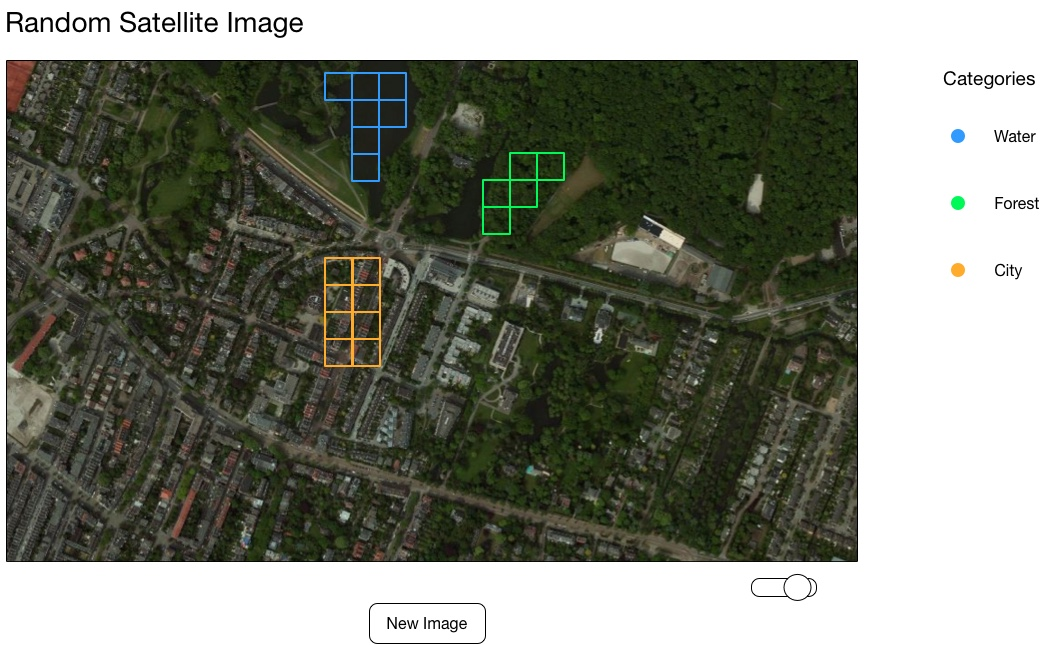
\includegraphics[width=0.8\textwidth]{./images/impression_toggle.jpg}
    \caption{Impression of what the user interacts with and a possible outcome.}
	\label{fig:impression}
\end{figure}
\noindent
The most notable attention grabber is the satellite image. This image will be acquired through a random call from a homogeneous satellite image database on every new instantiation of the system. Another possibility to acquire new data is by clicking on the 'New image' button. Right of the satellite image one can see labels (Forest, City, Water) which correspond with the labels which are outputs of the classification. Results obtained from our algorithm, given the current satellite image as input, are graphically fed back to the user. The impression above does that by showing a correspondence between image patches (squares) and their respective label via color coding laid over the satellite image. This rendition just shows a few islands of results as an example. Normally the entire image will have such arching.\\
\\
In order to classify the satellite image, the map is first divided into patches of predetermined dimensions. These patches are squares, the dimensions should be divisible by $2$ (as will be explained later) and these are the main, large patches to be fed into the neural network to be classified. The network will label the patches and return the outcome. The outcome is then evaluated to be rendered like is shown in Figure \ref{fig:impression}.\\
\\
However, we wanted to give the user the choice of making a more detailed classification with a smaller grid size without altering the workings of the neural network. To do so, an additional grid overlay is created with a small modification to the original rendering algorithm: the large patches now overlap each other in both dimensions by a half (hence that the large patches should be divisible by $2$). So if the map can be divided into N large patches in the width and M large patches in the height, this new setup will now have $(2N - 1)$ patches in the width and $(2M - 1)$ patches in the height, discarding patches that are halfway out of bounds. These patches are then fed to the neural network in the exact same fashion as the previous method. A second grid overlay is then effectively created, with the size of these smaller patches exactly a quarter of the larger patches. 
Figure \ref{fig:grid} provides a visual aid of this process, with the green patch indicating the large patch and the red patch indicating the resulting smaller patch.\\
\\
The idea is to link these smaller patches to its four larger patches. These are its labeled parents. The labels of the parents were determined by the network by giving it a certainty between 0 and 1 for each class, with 1 the highest certainty this patch belonged to the corresponding class.
A weighted majority vote is then used by summing the values of these classification of each of the four parents, grouped by their classes. The highest sum will be picked as the winner of the majority vote and its corresponding class will be used as a label for the smaller patch.\\
\\
For example, if there are three possible classes, $A$,$B$ and $C$, the certainty values of a patch can be denoted as $\{a_i, b_i, c_i\}$ where $1 \leq i \leq 4$. The values of the four parents of a small patch are then weighted, so you end up with $\{ \frac{1}{4}\sum_{i=1}^{4} a_i, \frac{1}{4}\sum_{i=1}^{4} b_i, \frac{1}{4}\sum_{i=1}^{4} c_i\}$. Whomever is biggest, wins. Doing this for all $(2N - 1) \times (2M - 1)$ patches results in a new classification grid showing more detail. This in turn allows the user to make a finer classification and switch back and forth accordingly via the toggle button displayed in the impression of Figure \ref{fig:impression}.

\begin{figure}[h!]
    \centering
    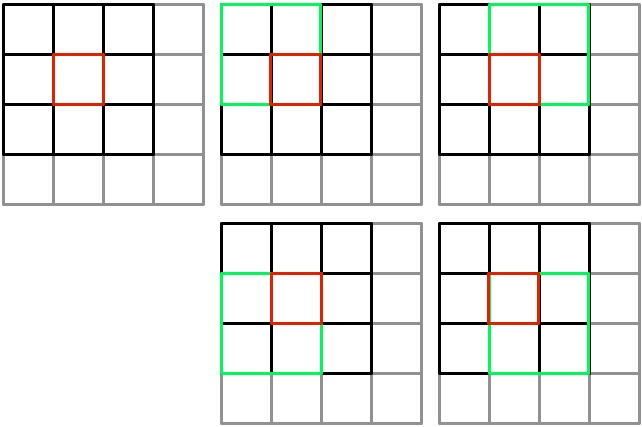
\includegraphics[scale=0.6]{./images/grid_explained.jpg}
    \caption{Grid structure which facilitates the algorithm, green denotes a large patch, while red denotes the small patch. Here is illustrated how the red, smaller patch has four green, larger parent patches.}
	\label{fig:grid}
\end{figure}

\section{MoSCoW}
Since our time to work on this project is limited while the amount of goals we wanted to accomplish in this period were numerous, we used the MoSCoW analysis technique to prioritize these goals and focus on the most important requirements. MoSCow stands for \textit{Must have}, \textit{Should have}, \textit{Could have} and \textit{Would have}, with the importance of each category ordered in a descending fashion. This enables us to identify core requirements which are absolutely necessary for the functionality of our implementation and in turn enables us to set up the core functionality first before focusing on the secondary objectives. All the requirements are labeled in these four classes. These requirements were laid out before the concept we eventually pursued had taken shape.\\

\subsection{Must have}
Must have requirements are critical to project success. 
\begin{itemize}
\item Create code based on a \textit{Convolutional Neural Network} (CNN) that enables automatic classification of patches from satellite images. Considering images acquired on provincial level and a substantial amount of pixels in one patch (at least 50 x 50 pixels). 
\item At least the following classes should be recognized: vegetation, city and water. 
\item Develop a way to visualize the automatic classifications clearly.
\end{itemize}

\subsection{Should have}
Requirements labeled as `Should have' are important to book success, but not necessary for delivery.

\begin{itemize}
\item Create a clear interface in which the unlabeled images can be uploaded, and the output consists of labeled images. 
\item Calculate the uncertainty in the classification and ask user input for very uncertain patches.
\end{itemize}

\subsection{Could have}
It would be very nice if we would be able to reach the Could have features, but they are not critical. 
\begin{itemize}
\item Experiment with preprocessed images (noise reduction, gradient calculations)
\item Analyze images on city level, so with more details present. For this purpose new classes have to be added, such as roadways, cycle paths, 	buildings, distinct vegetations etcetera. 
\item Experiment with other models than the state-of-the art \textit{LeNet-1 CNN}. For examples, a CNN in which \textit{Genetic Algorithms} are incorporated, or implementing an \textit{Extreme Learning Machine} for the training of the weights. 
\end{itemize}

\subsection{Would have}
These requirements are implemented only in the most ideal situation. They are considered as the dream project, sometimes serving as a suggestion for further projects. 

\begin{itemize}
\item Develop a method for high-detailed automatic vector graphics, in which segmentation of the distinct labeled classes is incorporated.
\item Use the input of the users to improve the automatic classification. 
\item Sell the software package to Google. 
\end{itemize}

\subsection{Evaluation of the requirements}
Now that the implementation has been finished, it is time to evaluate the whether the requirements were met. This, too, will be done in accordance with MoSCoW.\\
\\
\textbf{Must have}\\
As the name of the Must have category implies, these requirements are critical to the success of the project and as such, these requirements were all met. The CNN is designed and is trained beforehand, the resulting weights are then injected into the CNN placed on the server, used to classify the map patches. The CNN is capable of distinguishing three separate classes, with an experimental CNN capable of distinguishing four classes (further elaborated on in Section \ref{chap:resultsanddiscussion}).
A basic web interface was created, with the ability to highlight specific classes to help visualize the classification of the network.\\
\\
\textbf{Should have}\\
Due to time constraints, some requirements had to be modified in order to implement them or were left out altogether. The ability to upload own satellite imagery was replaced with the ability to acquire random satellite imagery of Amsterdam and its surroundings, which are in turn classified by the network. Choosing this route means that we can worry less about content validity and security of the application. The calculation of uncertainty is possible, but the implementation of user correction in conjunction with this uncertainty was left out. This is due to time constraints and the fact that we have not implemented on-line learning, but rather let the network train off-line beforehand, making this feature obsolete.\\
\\
\textbf{Could have}\\
Preprocessing the images could have been implemented and would surely boost our classification results. However, the goal of this project was not to achieve a high classification performance, but rather to implement a neural network that could learn on its own what the best discriminating features of an image is. The option to classify maps on different altitude levels is not implemented, also due to time constraints. Different levels of altitude means to either have a general neural network that works on all altitudes, or having to train the network on different altitudes in order to produce multiple weight setups. Both of these options meant more time needed to develop, implement and test the new setups. We did manage to implement a good general neural network, but we did not have time to test this functionality properly on different altitudes. Different setups have been experimented with, which will be discussed in Section \ref{chap:resultsanddiscussion}.\\
\\
\textbf{Would have}\\
The would haves requirements were on a whole different level and thus are self-explanatory why they weren't implemented.

\chapter{System design}
\label{chap:softwarearchitecture}
A plan has been established what kind of application should come about. The previous discussion pressed for a certain kind of structure. One where a Neural Network is central to the problem to be solved. But also a frontend is needed for certain user interaction as well as an infrastructure in the backend which facilitates the communication with said frontend. This chapter discusses the infrastructure setup, the technologies used and the data being acquired.

\section{Infrastructure}
The impression given above in Figure \ref{fig:impression} is close to what the end result of the implementation will look like (although it only displays a certain state). Yet an entire infrastructure outside of the Neural Network is needed to facilitate the application. Below in Figure \ref{fig:communication} an infrastructure is visualized via the communication of the two entities.

\begin{figure}[h!]
    \centering
    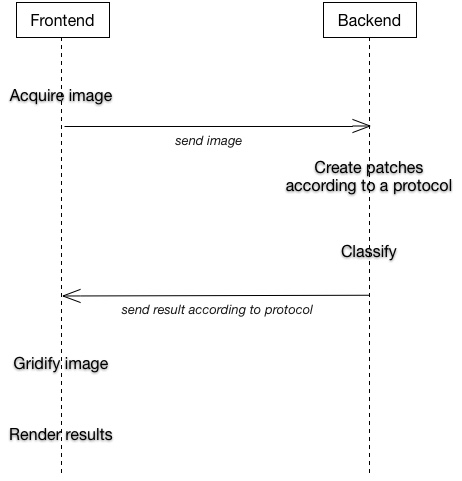
\includegraphics[scale=0.5]{./images/communication2.jpg}
    \caption{Communication visualization between front end and back end.}
	\label{fig:communication}
\end{figure}
\noindent
First, at the frontend, an image is acquired by the user from a map API call. The image is immediately send to the backend. There, patches are extracted according to a certain protocol (specific size and sequence) which also depend on whether small or large patches need to be visualized. The patches are classified by our Neural Network. Send back to the frontend are the label results in a list according to the sequence defined by the protocol mentioned earlier. Back at the frontend the image is made into a grid which also corresponds to the size and sequence of the protocol. The squares in the grid are then colored in according to the labels in the list that had been sent back.

\section{Technical Details}
The fronted consists of a web based interface, capable of visualizing the map acquired with the Bing Maps API \cite{bing}, the controls enabling the user to interact with the system and the resulting classification. The web application runs on Node.js and ZeroRPC. Node.js is an event-driven I/O server-side JavaScript environment and ZeroRPC is a cross-language RPC library, capable of performing remote procedure calls. Using these calls, we can effectively communicate with the Neural Network, written in Python, which is hosted on another server. The idea of this setup was to make it scalable: the initial plan was to implement the Neural Network with the idea of online learning, meaning the network could use a considerable amount of resources while running. If this network was hosted on the same server as the web server, this could be detrimental to the performance of both services.

\section{Map dataset}
The image which is being acquired every time comes from the Bing Maps database \cite{bing}. A predefined size of the map with satellite view enabled, the labels turned off, no other controls or logos visible and where the hight is set to 100 meters is put in the frontend.  Randomly a location inside the Amsterdam area is generated. Now the actual screengrap is taken from this acquired map.\\
\\
For training, satellite images from the same source and practice mentioned above are drawn on a per category/label basis. Meaning: specific images of locations only showing one category (water, forest, city) are being taken. Then patches are acquired code-wise over those images so that for each patch it is known what category/label belongs to it. These images are, however, taken from a larger corpus than the Amsterdam area, from across the world.

\chapter{Convolutional Neural Network}
\label{chap:CNN}
During our research phase, we encountered a variety of papers that describes the use of image classification based on Neural Networks. Most of these papers have one thing in common which is the use of Convolutional Neural Networks (CNN) \cite{Hongsheng2014} \cite{Farabet2013}. Since convolution operations are widely used to extract features from images and since these operations can be represented in terms of a Neural Network, these properties lead to the existence of the Convolutional Neural Networks.
\\\\
In general a CNN architecture consist of multiple convolution layers and sub-sampling layers. It depends on the architecture how these layers are followed by each other. The convolution layer is the layer which results after the convolution operator is performed by the convolution kernel. Since the goal is to extract general features from our input image we want the CNN to generalize. This generalization is partly realised by dimension reduction. Since convolution operation reduce the dimension of our input map with $\frac{M-N+1}{M}$, where $N$ is the dimension of the convolution kernel and $M$ the dimension of the input map, we want the dimension to be reduced more quickly. This is done by sub-sampling kernels which in general 'squeeze' or average the input map with a certain dimension. This operation is equivalent to a convolution operation but with a larger step-size (convolution uses a step size equal to 1) and equal weights for each element in the sub-sampling kernel.

\section{LeNet-1}
The model we implement is LeCun's LeNet-1 \cite{lenet}. This model uses an alternating sequence of convolution and sub-sampling layers. The architecture of this network is shown in Figure \ref{fig:Architecture}. The convolution layers act as feature maps, they consist of a window of a certain size, whose pixels are trainable weights. The sub-sampling layers reduce the dimensionality of the outputs. 
\begin{figure}[h!]
    \centering
    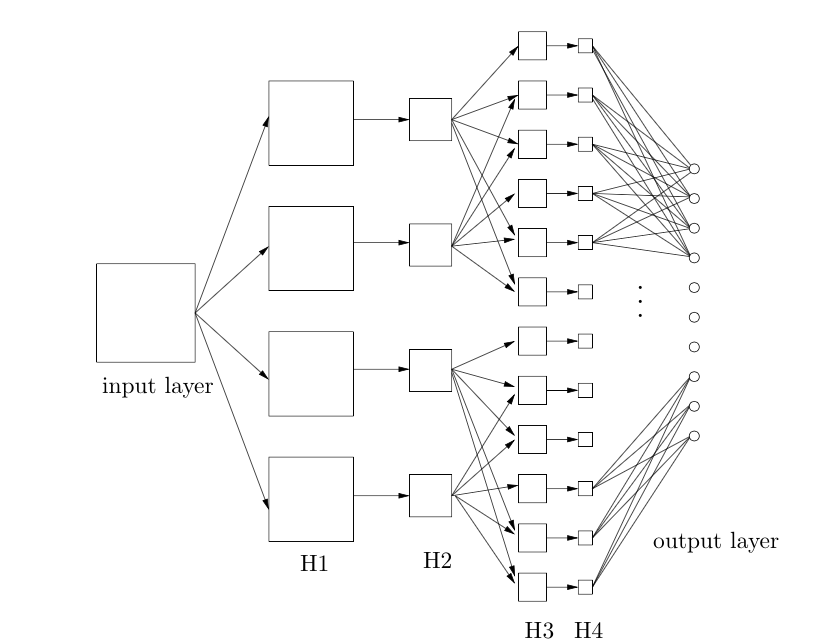
\includegraphics[scale=0.4]{./images/Architecture_CNN.png}
    \caption{The architecture of the CNN proposed by LeNet. H1 and H3 are the convolution layers, H2 and H4 the sub-sampling layers to reduce the dimension. }
	\label{fig:Architecture}
\end{figure}
\\\\
One of the biggest advantages of using CNN, and especially LeCun's LeNet-1 implementation, is the incorporation of backpropagation learning. Meaning that all the weights of the layers are adjusted iteratively, eliminating the need to manually create the convolution masks.
\\
\section{Backpropagation}
\label{sec:BP}
To train the network we have to adjust several parameters in the network. In this research we consider backpropagation from layer output to H4 to H3. In the whole network we use the Sigmoidal activation functions which is given by:
\begin{equation}
f(x)=\frac{1}{1+e^{-x}} 
\end{equation}	
The error function is defined as:
\begin{equation}
E=\sum_{k} \frac{1}{2}|t_k-F_{k}|^{2}
\end{equation}
Where $t_k$ represent the labeled class of the training and $F_{k}$ is the corresponding activation of the classifier neuron . This variable is $1$ if the corresponding class is trained and $0$ if this is not the case. Below the functions are listed in which we go from the activation of our classifier neuron to weights present in layer H3. In these equations $r$ stands for row which is the first branch after the first convolution i.e. the total rows is equal to the amount of different feature maps in H1. $b$ stands for the amount of branches per row. $k$ stands for the amount of classes which are trained by the network.
\begin{equation}
\begin{split}
	&F_{k}= f( x_{k}) \\
	& x_{k}=\sum_{ij} W^{4rbk}[i,j] \; H^{4rb}[i,j] - b_{k} \\
	&H^{4rb}[i,j]= \sum_{u,v} W^{3rb}[u,v] \; H^{3rb} [2i+u,2j+v] \\
	&H^{3rb} [2i+u,2j+v]= f\left (x^{3rb}[2i+u,2j+v] \right) \\
	&x^{3rb}[2i+u,2j+v]=\sum_{nm} W^{2rb}[n,m] \; H^{2rb}[n+(2i+u),m+(2j+v)] -b^{3rb}
\end{split}
\end{equation}
In the above equations $i$ and $j$ are the row and column respectively for the elements in the output maps and end-weight matrix $ W^{4rbk}$. The superscript in the latter indicates for layer H4 and corresponding row $r$ and branch $b$. The elements $u$ and $v$ are the elements over the sub-sampling kernel where $n$ and $m$ are the elements over convolution kernel $W^{2rb}$. From these equations we can calculate the update-rules for backpropagation. This is done by applying the gradient descent method in which we calculate the derivatives of the error function. The update-rule consists of the derivative with respect to the parameter we want to update.  
\\\\
For updating $W^{4rbk}$, also called the end-weights, we use:
\begin{equation}
\begin{split}
\Delta W^{4rbk}[i,j]&= \sum_{k} - \eta \frac{dE}{d F_{k}} \frac{dF_{k}}{dx_{k}} \frac{dx_{k}}{dW^{4rbk}[i,j]} \\
&= \sum_{k} \eta (t_{k}-F_{k})\frac{e^{-x_{k}}}{(1+e^{-x_{k}})^{2}} \frac{dx_{k}}{dW^{4rbk}[i,j]} \\
&= \eta (t_{k}-F_{k})\frac{e^{-x_{k}}}{(1+e^{-x_{k}})^{2}} H^{4rb}[i,j]
\end{split}
\end{equation}
For updating the bias $b_{k}$ corresponding to each classifier neuron:
\begin{equation}
\begin{split}
\Delta b_{k}= - \eta \frac{dE}{d F_{k}} \frac{dF_{k}}{dx_{k}} \frac{dx_{k}}{b_{k}}=\eta (t_{k}-F_{k})\frac{e^{-x_{k}}}{(1+e^{-x_{k}})^{2}} (-1)
\end{split}
\end{equation}
The updating for the elements in the convolution kernel $ W^{2rb}$ requires some more derivatives:
\begin{small}
\begin{equation}
\begin{split}
	&\Delta W^{2rb}[n,m] = \\
	&\sum_{k} - \eta  \frac{dE}{dF_{k}} 
	\frac{dF_{k}}{dx_{k}} 
	\sum_{ij} \frac{dx_{k}}{dH^{4rb}[i,j]} 
	\sum_{uv}\frac{dH^{4rb}[i,j]}{d H^{3rb} [2i+u,2j+v]} 
	\frac{d H^{3rb} [2i+u,2j+v]}{d x^{3rb}[2i+u,2j+v]}
	\sum_{nm}\frac{d x^{3rb}[2i+u,2j+v]}{d W^{2rb}[n,m]} \\
	=&\sum_{k} \sum_{ij} \sum_{uv} \sum_{nm}  \eta (t_{k}-F_{k})\frac{e^{-x_{k}}}{(1+e^{-x_{k}})^{2}} W^{4rbk}[i,j]  W^{3rb}[u,v] \frac{e^{-x^{3rb}[2i+u,2j+v]}}{(1+e^{-x^{3rb}[2i+u,2j+v]})^2} \\
	 & H^{2rb} [n+(2i+u),m+(2j+v)]
\end{split}
\end{equation}
\end{small}
Since there is also a bias $b^{3rb}$ present in layer H3 we have to update these weights as well:
\begin{small}
\begin{equation}
\begin{split}
	&\Delta b^{3rb} =\\
	&\sum_{k} - \eta  \frac{dE}{dF_{k}} 
	\frac{dF_{k}}{dx_{k}} 
	\sum_{ij} \frac{dx_{k}}{dy^{4rb}[i,j]} 
	\sum_{uv}\frac{dy^{4rb}[i,j]}{d y^{3rb} [2i+u,2j+v]} 
	\frac{d y^{3rb} [2i+u,2j+v]}{d x^{3rb}[2i+u,2j+v]}
	\frac{d x^{3rb}[2i+u,2j+v]}{d b^{3rb}} \\
	&=\sum_{k} \sum_{ij} \sum_{uv} \eta (t_{k}-F_{k})\frac{e^{-x_{k}}}{(1+e^{-x_{k}})^{2}} W^{4rbk}[i,j]  W^{3rb}[u,v] \frac{e^{-x^{3rb}[2i+u,2j+v]}}{(1+e^{-x^{3rb}[2i+u,2j+v]})^2} (-1)
\end{split}
\end{equation}
\end{small}
\begin{small}
\begin{equation}
\end{equation}
\end{small}


\chapter{Method}
\label{chap:method}
The architectures of the Convolutional Neural Networks we use for this research are based on the LeNet-1 described in chapter \ref{chap:CNN}. The architectures could differ in several ways from each other. First, we can adjust the sizes and types of the first convolution kernels. Second, the dimension reduction for both sub-sampling kernels can differ. The size of the second convolution kernels can be changed and the dimension of the output map (H4) can be chosen differently. At last, the amount of classifier neurons at the end of the network can be modified but this necessarily depends on the amount of classes the network has to resolve.  It is possible to vary more parameters for these networks but this research is limited to these cases. 
\\\\
To investigate which architectures are sufficient to use for our application a few architectures were explored. The various parameters as described above are changed resulting in different network designs. These networks can be trained in two different ways: backpropagation on the classifier neuron biases ($b_{k}$) and end-weight ($ W^{4rb}$) or the latter and further backpropagation where also the weights of the second convolutional kernels are trained ($ W^{2rb} $) and their biases ($b^{3rb}$). First we investigated how the networks perform when we only do the first type of training since further backpropagation will be more computationally expensive. Their performance is measured with a method based on cross-validation (see appendix \ref{app:DiffentArchitectures}). 
\\\\
\textbf{Marjo: hier jouw stuk over hoe jij je resultaten hebt verkregen. En ook iets over die RGB brightness. }
\\\\
The networks were programmed in \textit{Python}. No special packages related to Neural Networks were used such as \textit{Theano}. For the convolution operation we used a package \textit{Scipy.signals} which contains a convolution function. Furthermore, some additional packages were used for basic operations in the program such as \textit{Numpy} and \textit{PIL}. The latter is used to import images for the root. Since we use patches to train the network we write a function which divides the imported images in patches. Each patch get the label corresponding to the class it belongs to so it can be used to train the network. The images were obtained from Bing Maps \cite{bing}. Suitable images were gathered by selecting only places (all around the world) which contains the favored class. A side note has to be included for the images with the class city since these images may include some tree, grassland or water patches and thus will be labeled with the class city. Most other classes forest, grassland and water does not entail this problem since a great proportion of the world purely contains these classes.



\chapter{Results and Discussion}
\label{chap:resultsanddiscussion}
In the first phase of our research we made a convolutional neural network based on LeNet-1. We experimented with different convolution kernels in the first layer (H1) of the network and differed the amount of branches in the third layer (H3). We started with manually chosen convolution kernels for both layers H1 and H3. We began with input patches of 50 x 50 followed by a convolution kernel of 5x5 resulting in a feature map of dimensions 46x46. Next, sub-sampling with a dimension reduction of 2 results in a feature map of dimension 23x23. Again we did different 4x4 convolution kernel operation creating branches in H3 resulting in 20x20 feature maps. Sub-sampling with a dimension reduction of 5 resulted in an 4x4 output map. These output maps are then connected to two different classification neurons for Forest and City. \\\\
We used the Sigmoid function as activation function only for our classification-neurons. Thus, no activation functions were used earlier in the network (compared to LeNet-1). We performed backpropagation on the weights connecting the output maps with the classification neurons and biases. The first functioning results where found with 4 feature maps in H1 and 2 feature maps in H3 each where the network was enabled to recognize some forest/city patches from an new image. These results were too poor to include in this report. We used the convolution kernels shown in figure \ref{fig:firstFilters}. The Network was trained on structure only so no color features were included. 
\begin{figure}[bth!]
	\centering
	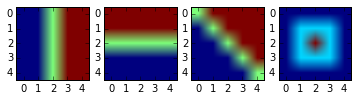
\includegraphics[width=0.5\textwidth]{./images/firstFilters.png}
	\caption{The four filters used in the first stage where the CNN was able to distinguish forest and city.}
	\label{fig:firstFilters}
\end{figure} 
\\\\
In the second phase we tried to extend our classes with the class \textit{water} or \textit{grassland}. From the first few runs it turned out that the networks found it hard to distinguish the classes \textit{forest} and \textit{water}. By comparing some patches of both classes it became quite evident that this distinction is hard since there structure is similar (see Figure \ref{fig:WaterForestPatch} ). For this reason we included the class \textit{grassland} instead of \textit{water}. From figure \ref{fig:GrassForestPatch} we can see that these patches are less similar and thus we would expect the network to perform better on these these combination of classes.
\\\\
During this phase we tried to investigate whether training only the end-weights ($W^{4rb}$) and biases ($b_{k}$) were sufficient to train the network to classify three classes. We experimented with different types of architectures for the networks. We trained nine networks with different sub-sampling operations. Also the sizes of the convolution kernels and the dimension of the output maps were varied. Each network was trained two times to get an idea how its performance is. To get statistical significance we should train each network multiple times but due to high computational costs we limited the amount of trainings per network at two. To see the results and the method used to evaluate these performances the reader is referred to appendix \ref{app:DiffentArchitectures}. Although, the results can not be statistically justified we can obtain some properties from these findings. By comparison of network 1 with network 8 we can see that similar amount of trainable weights does not correspond with similar performance. Network 1 consists of 189 trainable weights (excluding the bias) and Network 8 has 192  trainable weights but the performance of the latter is much lower. The same holds for a comparison of Network 2 with Network 3 (or Network 6). However, the overall performance of networks with more trainable weights perform better. Furthermore, it also turns out some Networks are able to recognize almost $75$ \% correct (see Networks 4,7 and 9 ). 
\\\\
\textbf{Marjo: Justification waarom we RGB values hebben meegenomen? En jouw resultaten uiteraard. }
\begin{figure}[bth]
	\centering
	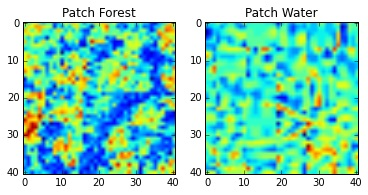
\includegraphics[width=0.5\textwidth]{./images/WaterForestPatch.jpg}
	\caption{A forest and water patch are shown. Their similarity makes it hard for the CNN to distinguish these two classes.}
	\label{fig:WaterForestPatch}
\end{figure}
\begin{figure}[bth!]
	\centering
	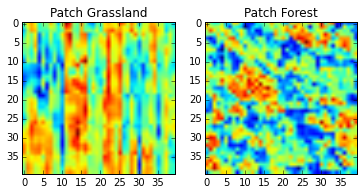
\includegraphics[width=0.5\textwidth]{./images/GrassForestPatch.jpg}
	\caption{A grassland and forest patch are shown.}
	\label{fig:GrassForestPatch}
\end{figure}
\\\\


\chapter{Personal Contributions}
\label{personalcontributions}
\section{Michiel Bongaerts}
During the project my focus was on the implementation of the Convolutional Neural Networks in Python. I programmed the first design of our CNN based on LeNet-1 with only backpropagation in the end-weights. I gathered images from Bing maps for the different classes to train this CNN on. It turned out that this first design (qualitatively) worked for unknown input images where it could distinguish between forest and city. This results encouraged us to continue with the CNN architectures. Next, I focused on the backpropagation algorithm in which the CNN was able to backpropagate further till the weights of the second Convolution kernel. This algorithm turned out to be very computational expensive which stagnated my research on this. I continued to evaluate different kinds of architectures. 

\section{Tung Phan}
I was responsible for the back end implementation, finding the right tools and setting up the communication between Python and JavaScript. Maniek and I also worked on creating an algorithm for the smaller grid patch system. Because the exact dimensions of the initial patches fed to the neural network is extremely important, simply resizing them to a smaller dimension to create a finer classification was not an option. Instead, we created the smaller grid algorithm. The smaller patches had to be linked to their 'parent' patches, allowing us to determine the label of the smaller patch by a weighted majority vote. This in turn allowed us to make a more accurate classification without being heavily dependent on the initial patch dimensions. I was also partly involved with the front end, together with Maniek. Of course, during the project, I also discussed the architecture of the CNN and helped brainstorming, though Marjolein and Michiel did most of the heavy lifting on that side.

\section{Maniek Santokhi}
My contribution first started with the implementation of the frontend. Mainly the part that receives the input according to a protocol which in turn is being rendered into colored interactive squares. The first implementation contained a map from Google, but Bing showed more versatility. Together with Tung we devised and implemented (both at the front- as well as the backend) the algorithm that facilitates the toggling between the finer and more coarser grid that shows the classification results. Although a straightforward idea, this proved tedious during implementation. With Michiel we brainstormed and tried out different convolution filters as a means to improve the classification results. Overall I participated in the general discussion regarding the different CNN implementations. As usual with software creation, bug fixing and general refinements is something I also concerned myself with.

\bibliography{Report}
\bibliographystyle{apacite}



\begin{appendices}
	
\chapter{Evaluation of different CNN architectures}
\label{app:DiffentArchitectures}
To compare the different architectures we used a cross-validation based method. This includes the training of the network on 90\% of the data/total amount of patches. The remaining 10\% is used to validate the performance of the network. The training was performed in three steps. In the first step the learning rates were quite high such that the network roughly learns to recognize the classes. The following steps were trainings in which the learning rates were smaller. In other words, we did not use decaying learning rates or another method. Backpropagation  was only applied to the end-weights $W^{4rb}$ and the biases $b_{k}$. To summarize, each patch from the (90\%) training set  has been 'seen' by the network three times and each time with a different learning rate. 
\\\\
From the network we want to know how it performed in general and on each class. So from the cross-validation the following values were subtracted: general performance and the performance on each class. Since this validation is executed for three classes we obtain these four values. The values are calculated by the relative fraction of patches which were classified correctly, or:
\begin{equation}
\label{eq:P}
P= \frac{N_{right}}{N_{right}+ N_{wrong}}
\end{equation}
In which $N_{right}$ determines the number of correctly classified patches and $N_{wrong}$ the number of patches which were classified wrong. This equation is used to calculate the general performance in which we include all patches and for the performance for each class by only including the corresponding patches.
\\\\
All networks had similar convolution kernels for the first layer. If we used $3$ rows or convolution kernels in the first layer we used the kernel types shown in figure \ref{fig:3filters}. For the networks with $5$ and $7$ the kernels are shown in figure \ref{fig:5filters} and \ref{fig:7filters} respectively. The weights for the second convolution kernels were drawn from a uniform distribution and therefore these kernels differed for each network. With equation \ref{eq:P} the performances of the networks was calculated. The classifier neuron with the highest activation value is taken to be the class of classification. If this class matches the corresponding class of the input patch, the network is considered to evaluate the patch as correct, otherwise it is classified as wrong. Mind that city patches might include tree or grassland patches as well.

\begin{tiny}
	\begin{center}
		\begin{tabular}{| l |p{0.5cm} |p{0.5cm} |p{0.5cm} |p{0.75cm} |p{0.7cm} |p{0.7cm} |p{0.75cm} |p{0.75cm} |p{0.75cm} |p{0.5cm} |p{0.8cm} |p{0.8cm} |p{0.8cm} |r | }
			\hline
			Net	& Amount of rows	& Amount of branch	& Input patch size	& First Conv. Filter size	& Pooling	& Second Conv. Filter size (random)&	Pooling	&H4	& Tot. end-weights	&Tot. Training patches	& Cross validation 90\%-10\% & Forest &	City	& Grassland \\ \hline
			
			1&	7&	3&	40x40&	11x11& 	3&	5x5&	2&	3x3&	189&	21560&	0.638&	0.768&	0.759&	0.406 \\ \hline
			1&	7&	3&	40x40&	11x11&	3&	5x5&	2&	3x3&	189&	21560&	0.720&	0.745&	0.854&	0.548\\ \hline
			2&	5&	3&	40x40&	11x11& 	3&	5x5&	2&	3x3&	135&	21560&	0.674&	0.755&	0.805&	0.482\\ \hline
			2&	5&	3&	40x40&	11x11& 	3&	5x5&	2&	3x3&	135&	21560&	0.702&	0.833&	0.860&	0.416\\ \hline
			3&	5&	3&	40x40&	9x9&	4&	3x3&	2&	3x3&	135&	21560&	0.549&	0.875&	0.587&	0.202\\ \hline
			3&	5&	3&	40x40&	9x9&	4&	3x3&	2&	3x3&	135&	21560&	0.499&	0.685&	0.687&	0.138\\ \hline
			4&	5&	3&	40x40&	9x9&	2&	5X5&	3&	4x4&	240&	21560&	0.737&	0.610&	0.894&	0.713\\ \hline
			4&	5&	3&	40x40&	9x9&	2&	5X5&	3&	4x4&	240&	21560&	0.683&	0.709&	0.727&	0.608\\ \hline
			5&	7&	2&	40x40&	9x9&	2&	5X5&	3&	4x4&	224&	21560&	0.721&	0.630&	0.838&	0.694\\ \hline
			5&	7&	2&	40x40&	9x9&	2&	5X5&	3&	4x4&	224&	21560&	0.695&	0.712&	0.827&	0.541\\ \hline
			6&	5&	3&	40x40&	9x9&	2&	5X5&	4&	3x3&	135&	21560&	0.695&	0.795&	0.820&	0.465\\ \hline
			6&	5&	3&	40x40&	9x9&	2&	5X5&	4&	3x3&	135&	21560&	0.635&	0.819&	0.833&	0.257\\ \hline
			7&	5&	3&	40x40&	11x11& 	2&	4x4&	3&	4x4&	240&	21560&	0.700&	0.597&	0.781&	0.724\\ \hline
			7&	5&	3&	40x40&	11x11& 	2&	4x4&	3&	4x4&	240&	21560&	0.743&	0.705&	0.866&	0.650\\ \hline
			8&	3&	4&	40x40&	9x9&	2&	5x5&	3&	4x4&	192&	21560&	0.568&	0.351&	0.716&	0.628\\ \hline
			8&	3&	4&	40x40&	9x9&	2&	5x5&	3&	4x4&	192&	21560&	0.518&	0.066&	0.702&	0.788\\ \hline
			9&	5&	3&	40x40&	11x11& 	2&	8x8&	2&	4x4&	240&	21560&	0.737&	0.642&	0.848&	0.728\\ \hline
			9&	5&	3&	40x40&	11x11& 	2&	8x8&	2&	4x4&	240&	21560&	0.728&	0.720&	0.864&	0.601 \\ \hline
			
			
		\end{tabular}
	\end{center}
\end{tiny}	


\begin{figure}[bth!]
	\centering
	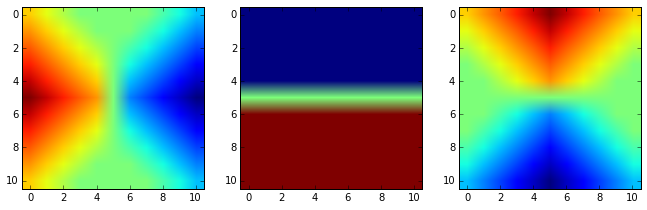
\includegraphics[width=0.3\textwidth]{./images/3filters.jpg}
	\caption{The three convolution kernels used for the architectures with three rows.}
	\label{fig:3filters}
\end{figure}

\begin{figure}[bth!]
	\centering
	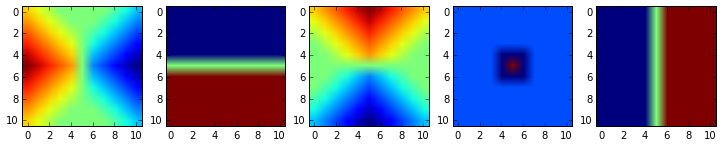
\includegraphics[width=0.5\textwidth]{./images/5filters.jpg}
	\caption{The five convolution kernels used for the architectures with five rows.}
	\label{fig:5filters}
\end{figure}

\begin{figure}[bth!]
	\centering
	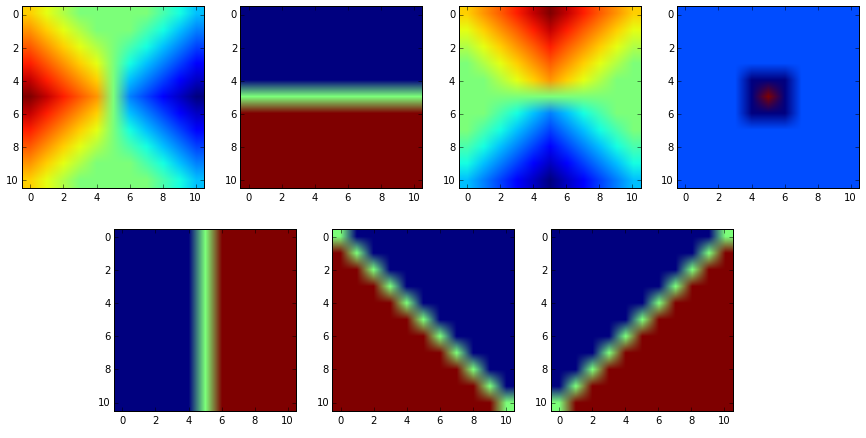
\includegraphics[width=0.4\textwidth]{./images/7filters.jpg}
	\caption{The seven convolution kernels used for the architectures with seven rows.}
	\label{fig:7filters}
\end{figure}

\end{appendices}






\end{document}



